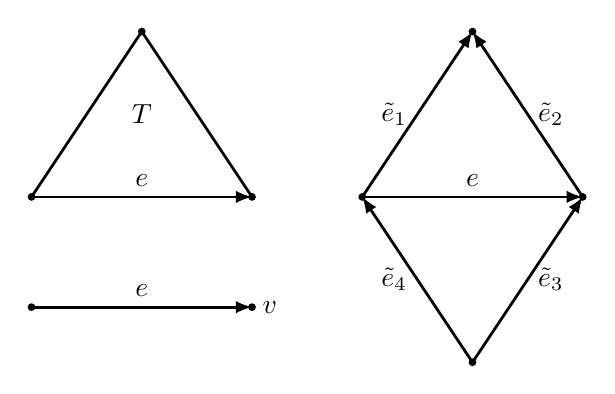
\begin{tikzpicture}[>=latex, line width=1pt, scale=0.7]

% vertex coords
\coordinate (V1) at (-2,0);
\coordinate (V2) at (2,0);
\coordinate (V3) at (0,3);
\coordinate (V4) at (0,-3);

%points
\fill(V1) circle(2pt);
\fill(V2) circle(2pt);
\fill(V3) circle(2pt);
\fill(V4) circle(2pt);

%arrows
\draw[->] (V1) -- (V2) node [midway,above] {$e$} ;
\draw[->] (V2) -- (V3) node [midway,right] {$\tilde{e}_{2}$};
\draw[->] (V1) -- (V3) node [midway,left] {$\tilde{e}_{1}$};
\draw[->] (V4) -- (V2) node [midway,right] {$\tilde{e}_{3}$};
\draw[->] (V4) -- (V1) node [midway,left] {$\tilde{e}_{4}$};



\coordinate (VV1) at (-8,0);
\coordinate (VV2) at (-4,0);
\coordinate (VV3) at (-6,3);

\fill(VV1) circle(2pt);
\fill(VV2) circle(2pt);
\fill(VV3) circle(2pt);

\draw[->] (VV1) -- (VV2) node [midway,above] {$e$} ;
\draw[] (VV2) -- (VV3) ;
\draw[] (VV1) -- (VV3) ;

\node at (-6,1.5) {$T$};



\coordinate (VVV1) at (-8,-2);
\coordinate (VVV2) at (-4,-2);

\fill(VVV1) circle(2pt);
\fill(VVV2) circle(2pt);

\draw[->] (VVV1) -- (VVV2) node [midway,above] {$e$} ;

\node[right] at (VVV2) {$v$};


\end{tikzpicture}
